\chapter{The Packing Algorithm}
\label{chap:packing}

This chapter describes how we can obtain a deterministic packing solution, i.e. a list of containers and boxes packed within them, 
from the packing input and the packing rules. The packing rules contain information regarding the rotation of each box, the heuristic that will
determine how the box is placed in the container, and the order in which the boxes are packed. 

First, the list of input boxes is converted into an ordered list of pending boxes using the packing rules.
Each pending box contains the input box together with the information about its rotation and the heuristic that will be used to pack the box. 

Once we have the list of pending boxes, they can be packed using the box packing algorithm that 
takes each pending box and tries to pack it into an open container chosen by the placement heuristic assigned to that particular pending box.
In case no fitting container and space are found, a new container is opened.
Once a pending box is placed into a container, we call it a placed box.
This placed box consists of the input box information, its rotation, the space it occupies within the container, and the identifier of that container. 

The solution is then a list of open containers, each with a list of placed boxes within that particular container.
Since we can assign fitness to each solution, and the packing rules and packing input determine a unique solution, we can also assign fitness to the packing rules themselves with regard to the packing input.

\begin{figure}[H]
    \centering
    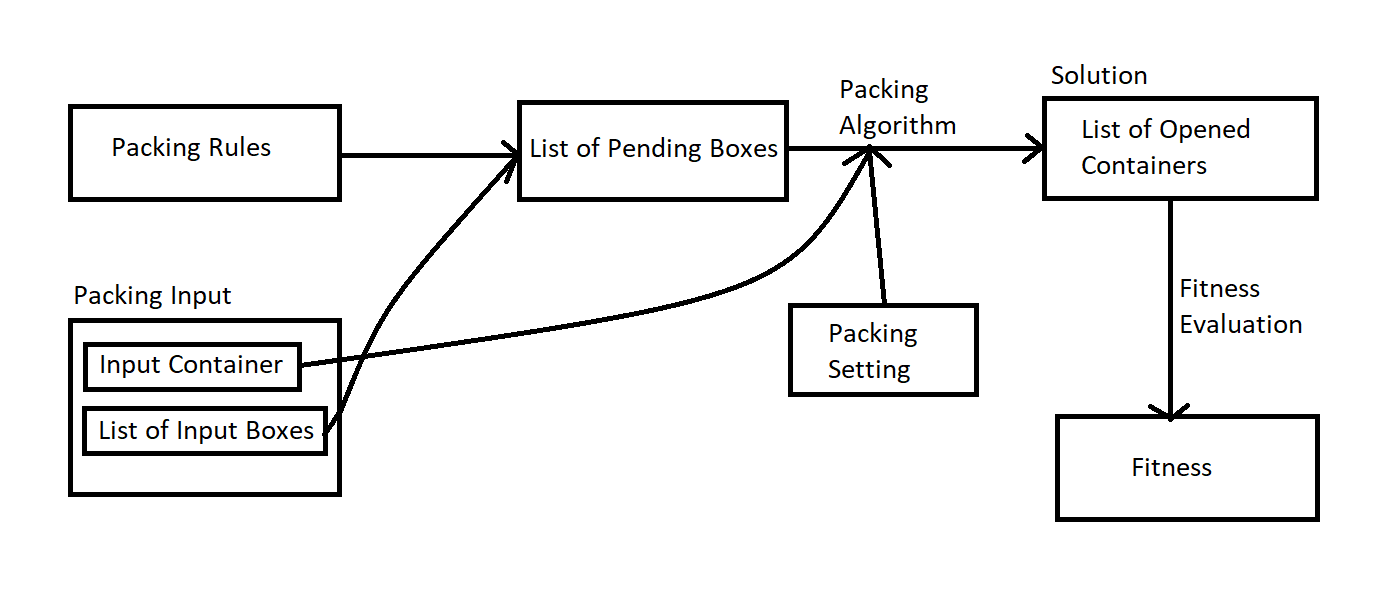
\includegraphics[width=1\textwidth]{img/Packing.png}
    \caption{
    }
    \label{fig:Packing Overview}
\end{figure}


\section{Terminology}

\subsection{Pending box}

A \emph{pending box} is represented as a triple $(B, Rot, H)$, where:
\begin{itemize}
    \item $B$ is the input box,
    \item $Rot$ is the selected rotation,
    \item $H$ is the placement heuristic.
\end{itemize}

The reason each pending box has its own placement heuristic, rather than using a single heuristic for all pending boxes, is to support variability in evolutionary algorithms.

\subsection{Placement Heuristic}

A \emph{placement heuristic} is a function that takes a list of currently opened containers and an input box with its rotation, 
and returns a selected container along with the region where the box should be placed.
Since the input is defined only as a list of opened containers, 
the heuristic has considerable flexibility. It can take into account various factors when choosing the target container and placement space. 
For example, if the heuristic had access only to the EMR lists of containers, 
its decision-making would be restricted to available empty regions. 
In this more general formulation, however, it can also consider additional attributes such as the weight or volume of each container.

If no valid placement for the box is found (i.e., there is no EMR in any container with sufficient dimensions, or placing the box would exceed the container's maximum weight), 
then the function returns \textit{null}.

\subsection{Opened Container}

An \emph{opened container} $C$ is represented as a triple $(C_{in}, B_c, EMR_c)$, where:
\begin{itemize}
    \item $C_{in}$ represents the input container,
    \item $B_c$ is the set of boxes already placed into the container,
    \item $EMR_c$ is the set of Empty Maximal Regions within the container.
\end{itemize}


\subsection{Placed Box}

A \emph{placed box} is represented as $(B, C, Reg, Rot)$, where:
\begin{itemize}
    \item $B$ is the box,
    \item $C$ is the container into which the box is placed,
    \item $Reg$ is the region occupied by the box within the container,
    \item $Rot$ is the rotation of the box.
\end{itemize}



\subsection{Packing Rules}

Let $\mathcal{H}$ denote the set of all available placement heuristics, and let $\mathcal{R}$ denote the set of all allowed box rotations.
The \emph{packing rules} provide a compact representation of the list of pending boxes and define the order in which they are packed. 
Formally, they are represented as a triple $(o, rot, h)$, where:
\begin{itemize}
    \item $o$ is a permutation list of integers from $1$ to $k$. 
    The value at index $i$ specifies the packing order of the box with identifier $i$.
    \item $rot$ is a list of length $k$, where the element at index $i$ represents the rotation assigned to the input box with identifier $i$, $rot \in \mathcal{R}^k$.
    \item $h$ is a list of length $k$, where the element at index $i$ represents the placement heuristic assigned to the input box with identifier $i$, $h \in \mathcal{H}^k$.
\end{itemize}
In other words, the packing rules determine the packing order, rotation, and placement heuristic for each input box, which together form the corresponding list of pending boxes.

\subsubsection{Vector representation}
In order to use the packing rules as an individual for the evolutionary algorithm, they can be represented as a continuous vector of length $3k$ consisting of real values in the interval $[0,1]$ \cite{goncalves2013}.
This vector is divided into three parts corresponding to the components $(o, rot, h)$.

In this triple, the first $k$ entries are sorted in ascending order to derive the permutation $o$, 
the second $k$ entries are interpreted as uniformly distributed indices to select elements from the set of allowed rotations $\mathcal{R}$, 
and the third $k$ entries are interpreted similarly to choose elements from the set of available heuristics $\mathcal{H}$. 
This transformation allows evolutionary algorithms to operate on the vector representation while still producing valid discrete packing rules.

If the set $\mathcal{H}$ contains only a single heuristic, the heuristic part becomes redundant, and the vector can be reduced to two parts with a total length of $2k$. 
A similar situation arises if rotations are not allowed, meaning that no rotation can be applied and the only feasible orientation is the default XYZ. 
In this case, the rotation part is unnecessary, and the vector can also be shortened to length $2k$. 
If neither of these parts are needed, the vector can be shortened further to length $k$. 
Furthermore, if the packing order is determined directly by a heuristic, the order part can also be omitted, as the order can be derived without relying on the packing vector.

\subsection{Packing Rules Fitness}
Previously, the concept of fitness was defined in the context of evaluating a solution. 
It is now evident that the packing input together with packing rules uniquely determine a specific solution. 
This allows fitness to be assigned not only to the solution itself but also to the packing rules with respect to the given packing input. 
The procedure is as follows: the packing rules are first converted into a list of pending boxes in a specified order, the packing algorithm is then applied to generate the solution, which is subsequently evaluated to determine its fitness.

\section{Empty Maximal Regions}

To keep track of unoccupied regions during the packing process, we assign each opened container a list of \emph{empty maximal regions} (EMR). 
An empty region is said to be \textit{maximal} if it is not a subregion of any other empty region. 
In the literature, the more common term is empty maximal spaces (EMS). However, the term regions is adopted here to ensure consistency with the terminology of this work \cite{lai1997, goncalves2013}.

Initially, each empty opened container $c$ has a single EMR, which is the region of the container itself, denoted as $R_c$. As boxes are placed into the container, the set of EMR is updated accordingly.

\subsection{Update of a Single Empty Maximal Region}

Assume we have an Empty Maximal Region:
\[
\text{EMR} = (\text{Start}, \text{End}) = ((x_s, y_s, z_s), (x_e, y_e, z_e))\text{,}
\]
and a region now occupied by a newly placed box:
\[
\text{BoxRegion} = ((x_b^s, y_b^s, z_b^s), (x_b^e, y_b^e, z_b^e))\text{.}
\]

If EMR and BoxRegion do not intersect, the original EMR remains unchanged.

If they do intersect, we define their intersection as:
\[
\text{IntersectRegion} = ((x_i^s, y_i^s, z_i^s), (x_i^e, y_i^e, z_i^e)) = \textit{EMR} \cap \textit{BoxRegion}\text{.}
\]

In the general case, this intersection splits the original EMR into up to six new EMR subregions, as follows:

\begin{itemize}
    \item \textbf{Left slab (along X)}:
    \[
    ((x_s, y_s, z_s), (x_i^s, y_e, z_e)) 
    \]

    \item \textbf{Right slab (along X)}:
    \[
    ((x_i^e, y_s, z_s), (x_e, y_e, z_e)) 
    \]

    \item \textbf{Front slab (along Y)}:
    \[
    ((x_s, y_s, z_s), (x_e, y_i^s, z_e)) 
    \]

    \item \textbf{Back slab (along Y)}:
    \[
    ((x_s, y_i^e, z_s), (x_e, y_e, z_e))
    \]

    \item \textbf{Bottom slab (along Z)}:
    \[
    ((x_s, y_s, z_s), (x_e, y_e, z_i^s))
    \]

    \item \textbf{Top slab (along Z)}:
    \[
    ((x_s, y_s, z_i^e), (x_e, y_e, z_e))
    \]
\end{itemize}

Each of these regions is only created if it has positive volume and satisfies the definition of a valid region, i.e., its start coordinates are less than or equal to its end coordinates in all dimensions.

When constraint C6 is applied, we have $z_b^s = z_s$, and thus the bottom slab is never created, reducing the number of new EMR to at most five.
Another consequence of constraint C6 is that the top slab must lie directly above the placed box. 
Therefore, its $x$ and $y$ coordinates are restricted to match the footprint of the box, making it more compact than in the general case:

\begin{itemize}
    \item \textbf{Top slab (along Z)}:
    \[
    ((x_i^s, y_i^s, z_i^e), (x_i^e, y_i^e, z_e)).
    \]
\end{itemize}

It is worth explicitly mentioning that there is no requirement for the newly generated EMR to be non-overlapping. Overlaps are allowed and common in this representation.

\subsection{Update of an Empty Maximal Regions List}

Since a newly placed box can intersect multiple EMR, it is necessary to update each region in the EMR list using the method described above. 
Once this is done, several additional steps must be taken \cite{goncalves2013}.

First, we check whether any of the newly created EMR is a subregion of another EMR in the list. Such subregions do not satisfy the definition of maximality and are therefore removed.
Second, we attempt to merge adjacent EMR that lie next to each other and start at the same height.
Due to constraint C6, each newly generated top slab lies directly above the placed box. 
However, the constraint still allows a box to rest on top of multiple smaller boxes, as long as its base is fully supported. 
This means that EMR starting at the same height and sharing a face can potentially be merged into a larger EMR.


\begin{figure}[H]
    \centering
    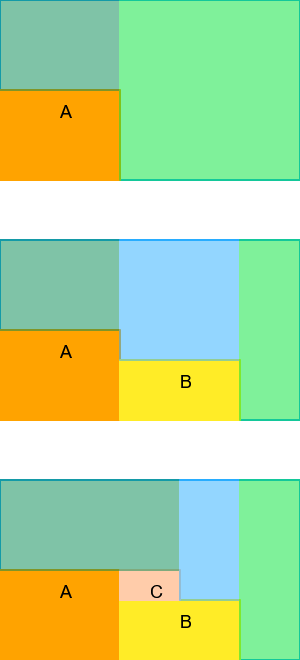
\includegraphics[width=0.45\textwidth]{img/SideEMR.png}
    \caption{Side view of EMR update. 
    Boxes are inserted sequentially in the order A, B, C. 
    The top EMR is always located directly above a box so that the support constraint is satisfied. 
    When two box tops are at the same height, as in the case of A and C, their top EMRs merge into a single EMR.}
    \label{fig:EMR-side-update}
\end{figure}

\begin{figure}[H]
    \centering
    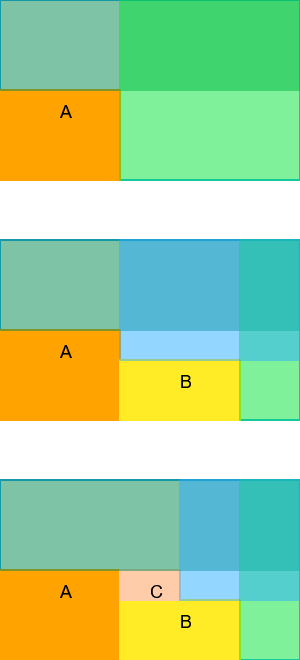
\includegraphics[width=0.45\textwidth]{img/TopEMR.png}
    \caption{Top view of EMR update. 
    Boxes are inserted sequentially in the order A, B, C. 
    Newly added boxes split existing EMR into several smaller regions, 
    and if any of these EMRs is a subregion of another EMR, it disappears. 
    For example, after inserting box C, part of the blue EMR becomes part of the dark green EMR.}
    \label{fig:EMR-top-update}
\end{figure}

\section{Heuristics}

\subsection{Order Heuristics}

If it is not desired for the evolutionary algorithm to determine the order of the boxes,the boxes can instead be pre-sorted using a simple ordering heuristic. 
In this case, the component of the packing rules responsible for ordering the boxes can be omitted.

The following predefined ordering heuristics are available in the algorithm:

\begin{itemize}
    \item \textbf{High Volume First:} Boxes are sorted by descending volume, placing the largest boxes first.
    \item \textbf{High Area Base First:} Boxes are sorted by descending base area (using rotated sizes), prioritizing those with the largest footprint.
    \item \textbf{High Weight First:} Boxes are sorted by descending weight, useful when container weight is often the limiting factor.
\end{itemize}

By using one of these heuristics, the packing order is fixed a priori and each box is placed according to the selected heuristic without relying on evolutionary selection for ordering. 
The evolutionary algorithm still operates, but its role is limited to selecting the rotations and placement heuristics for the boxes.

\subsection{Placement Heuristics}

The following heuristics are used in the experiments.

\begin{enumerate}

\item \textbf{Best Volume Fit} \\
This heuristic selects the EMR with the smallest volume that can still accommodate the box. 
The goal is to place the box into the tightest possible region in order to reduce fragmentation of the remaining free space.

\item \textbf{Max Distance} \\
For each feasible EMR, the Euclidean distance between the starting coordinate of the region and the far corner of the container is computed. 
The heuristic then selects the EMR that maximizes this distance. 

\item \textbf{Min X} \\
The heuristic selects the EMR with the smallest $x$ coordinate, i.e., it places the box as far as possible toward one side of the container. 
This produces more structured packings along the $x$ axis.

\item \textbf{Min Y} \\
This heuristic selects the EMR with the smallest $y$ coordinate and therefore prefers placements closer to the back side of the container.

\item \textbf{Gravity (Min Z)} \\
This heuristic selects the EMR with the smallest $z$ coordinate, which corresponds to placing the box as low as possible in the container. 

\item \textbf{Anti-Gravity (Max Z)} \\
In contrast to the previous heuristic, this strategy selects the EMR with the largest $z$ coordinate and therefore places boxes as high as possible in the container. 

\item \textbf{Bottom Left Back (BLB)} \\
This classical rule selects the EMR with the smallest $z$ coordinate. If several regions have the same value, the smallest $y$ coordinate is selected, and finally the smallest $x$ coordinate is used as a tie-breaking rule. 

\end{enumerate}

The set $\mathcal{H}$ is composed of a subset of the implemented heuristics chosen for a given instance, and during the evolutionary process, the algorithm selects which heuristic to apply for each box. 
If the size of $\mathcal{H}$ is one, i.e., only a single heuristic is available, the heuristic component of the packing rules is not needed, 
and each box is assigned this heuristic directly.

\section{The Box Packing Algorithm}

Given a list of ordered pending boxes, the algorithm iteratively attempts to place each box into one of the currently opened containers using a placement heuristic. 
If the box cannot be placed using its current rotation, the algorithm automatically tries all possible rotations. 
If no valid placement is found after considering all rotations, a new container is opened and the placement is attempted again. 
The algorithm continues in this way for all boxes. 
The pseudocode is shown in Figure~\ref{fig:box-packing-algorithm}.

\begin{figure}[htbp]
\centering
\begin{minipage}{0.95\linewidth}
\begin{algorithmic}[1]
\State \textbf{Input:} List of ordered pending boxes $\mathcal{B} = [b_1, b_2, \dots, b_n]$
\State \textbf{Output:} List of opened containers $\mathcal{C} = [c_1, c_2, \dots, c_m]$

\State Initialize empty list of opened containers $\mathcal{C} \gets []$

\For{each box $b \in \mathcal{B}$}

    \If{\textbf{TryPackBox}$(b, \mathcal{C})$ succeeds}
        \State continue
    \EndIf

    \If{\textbf{TryPackWithAnyRotation}$(b, \mathcal{C})$ succeeds}
        \State continue
    \EndIf

    \State Open a new container $c_{\text{new}}$
    \State Add $c_{\text{new}}$ to $\mathcal{C}$

    \If{\textbf{TryPackBox}$(b, \mathcal{C})$ succeeds}
        \State continue
    \EndIf

    \If{\textbf{TryPackWithAnyRotation}$(b, \mathcal{C})$ succeeds}
        \State continue
    \EndIf

    \State \textbf{Error:} Box could not be packed, may be too heavy or too large
\EndFor

\State \Return $\mathcal{C}$
\end{algorithmic}
\end{minipage}
\caption{Box Packing Algorithm Pseudocode}
\label{fig:box-packing-algorithm}
\end{figure}





